\chapter{Configuration Spaces}
% These definitions are presented in Abrams on page 10.
Given a topological space \(X\), the \(n\) point (topological) configuration space of \(X\) is
\(\Conf_n(X) = X^n - \Delta\) where \(\Delta\) is the diagonal in \(X^n\).

Treating a graph \(\Gamma\) as a topological space we can construct the
\(n\) point discretized or combinatorial configuration space \(\DConf_n(\Gamma)\) by 
% this diagonal needs elaboration.
removing a larger diagonal \(\Delta^{\square} = \{(e_1, \ldots, e_n) \mid x_i \cap x_j \neq \emptyset \text{ for some } i \neq j\}\)
from the cubical complex \(\Gamma^n\). Here \((e_1, \cdots, e_n)\) is any \(n\)-tuple of cells in \(\Gamma\).

Abrams in \cite{abrams2000configurationspaces} showed that \(\Conf_n(\Gamma)\) deformation retracts onto \(\DConf_n(\Gamma)\) is a cubical complex.
\begin{figure}
\centering
\begin{tikzpicture}
    \node (u1) at (2, 2) {\(u_1\)};
    \node (u2) at (4, 2) {\(u_2\)};
    \node (u3) at (3, 1) {\(u_3\)};
    \node (u4) at (3, 0) {\(u_4\)};
    \draw (u1) -- (u3);
    \draw (u2) -- (u3);
    \draw (u4) -- (u3);
\end{tikzpicture}
\caption{The \(Y\)-graph}
\label{fig:ygraph}
\end{figure}
In \cite{abrams2000configurationspaces} Abrams notes that any point in the
\(n\)-point configuration space is in one-to-one correspondence with a
collection of ``tokens'' placed on the graph. In this project, we will use a slightly different terminology and
and say ``particles'' placed on the graph instead.  Let \(\Gamma\) be the graph
in \ref{fig:ygraph} and consider \(2\) particles placed on \(\Gamma\) at \(u_1\)
and \(u_2\).  As the particle at \(u_1\) moves to \(u_3\), in the topological
configuration space the particle at \(u_2\) is free to simultaneously move to
\(u_3\) as well. However, both particles would not be able to occupy the vertex
\(u_3\) simultaneously.  In the combinatorial configuration space, as the
particle at \(u_1\) moves to \(u_3\), the particle at \(u_2\) can not move at
all since the edges \(u_1 u_3\) and \(u_2 u_3\) intersect at \(u_3\) and points
with coordinates belonging to both edges are thereby removed.

\begin{figure}
\centering
\begin{tikzpicture}
    \node (v1) at (0, 2) {\(v_1\)};
    \node (v2) at (0, 0) {\(v_2\)};
    \draw (v1) -- (v2);
    \node (u1) at (2, 2) {\(u_1\)};
    \node (u2) at (4, 2) {\(u_2\)};
    \node (u3) at (3, 1) {\(u_3\)};
    \node (u4) at (3, 0) {\(u_4\)};
    \draw (u1) -- (u3);
    \draw (u2) -- (u3);
    \draw (u4) -- (u3);
\end{tikzpicture}
\caption{An edge and a \(Y\)-graph}
\label{fig:edgeygraph}
\end{figure}
Consider the graph in figure \ref{fig:edgeygraph} and put particles at \(v_1\) and \(u_3\).
As the particle at \(v_1\) moves to \(v_2\) there are three ways that the particle at \(u_3\) can move.
Since each way that the particle at \(u_3\) can move can be done simultaneously as the movement of the particle at \(v_1\),
the \(1\)-cell corresponding to the movement of the particle at \(v_1\) to \(v_2\)
borders three distinct \(2\)-cubes (see figure \ref{fig:threepagebook}).
\begin{figure}
\centering
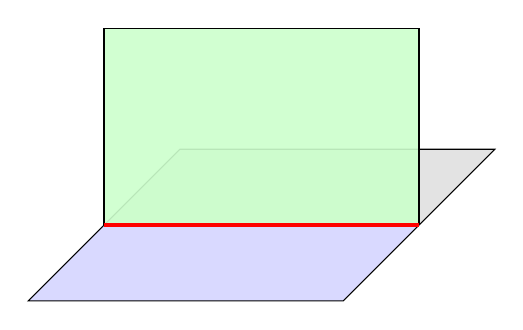
\begin{tikzpicture}
    scale=1.2,
    % Define a 3D-like perspective by setting the coordinate vectors.
    % x goes to the right, y goes up, and z gives a sense of depth.
    z={(-0.6cm,-0.4cm)}, 
    x={(1cm,0cm)},      
    y={(0cm,1cm)}       
]
    % --- Define Coordinates for the vertices of the book ---
    
    % The spine is a 1-cell from O to A
    \coordinate (O) at (0,0,0);
    \coordinate (A) at (4,0,0);

    \coordinate (B_Back) at (4,0,-2.5);
    \coordinate (C_Back) at (0,0,-2.5);

    \coordinate (B_Front) at (4,0,2.5);
    \coordinate (C_Front) at (0,0,2.5);

    \coordinate (B_Up) at (4,2.5,0);
    \coordinate (C_Up) at (0,2.5,0);

    % Draw book pages
    \fill[gray!30, opacity=0.75] (O) -- (A) -- (B_Back) -- (C_Back) -- cycle;
    \draw (O) -- (C_Back) -- (B_Back) -- (A);

    \fill[blue!20, opacity=0.75] (O) -- (A) -- (B_Front) -- (C_Front) -- cycle;
    \draw (O) -- (C_Front) -- (B_Front) -- (A);

    \fill[green!20, opacity=0.9] (O) -- (A) -- (B_Up) -- (C_Up) -- cycle;
    \draw (O) -- (C_Up) -- (B_Up) -- (A);


    % --- Draw the Spine on top so it stands out ---
    \draw[line width=1.5pt, red] (O) -- (A);

 
\end{tikzpicture}
\caption{A 3-page book}
\label{fig:threepagebook}
\end{figure}

Books are common structures found in configuration spaces.

% It would make so much more sense if we excluded the covers of the book when counting the pages.
% Then, a book with more than 0 pages is not homeomorphic to a surface. 
% However, this would be an annoying substitution in later proofs.
\begin{defn}
    An \(n\)-page book is a collection of \(n\) \(2\)-cubes each glued along a common edge.
    This edge is called the spine of the book.
\end{defn}
\begin{thm}
A book with more than \(2\) pages is not homeomorphic to a surface.
\end{thm}
\begin{proof}
Suppose there exists an \(n\)-page book which is homeomorphic to a surface but \(n > 2\).
Let \(S\) be the spine of the book and \(p\) be a point in the interior of \(S\).
Since the book is homeomorphic to a surface, there exists an open neighborhood \(U\) of \(p\)
which is homeomorphic to the disk \(D^2\). Let \(\phi\) be the homeomorphism from \(U\) to \(D^2\).
Notice that \(U \setminus S\) consists of \(n\) path components--one from each page of the book.
However,
\[
U\setminus S \cong \phi(U\setminus S) = D^2 \setminus \phi(S \cap U).
\]
\begin{figure}[h!]
    \centering
    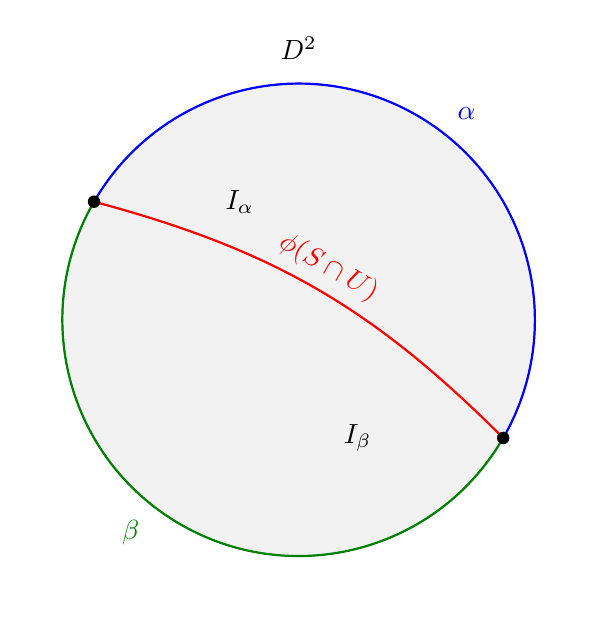
\begin{tikzpicture}[scale=1.5]
        % Define the main circle (the disk D^2) and fill it lightly
        \fill[gray!10] (0,0) circle (2cm);
        \draw (0,0) circle (2cm);
        \node at (0, 2.3) {\(D^2\)};

        % Define the start and end points of the arc on the boundary of the disk
        \coordinate (P1) at (150:2cm);
        \coordinate (P2) at (-30:2cm);

        % Draw the separating arc phi(S \cap U) with a distinct color
        \draw[thick, red] (P1) to[bend left=15] node[above, pos=0.5, sloped] {\(\phi(S \cap U)\)} (P2);

        % Draw the boundary path alpha
        \draw[thick, blue] (P2) arc (-30:150:2cm);
        \node[blue, above, xshift=18pt, yshift=-5pt] at (60:2cm) {\(\alpha\)};
        
        % Draw the boundary path beta
        \draw[thick, green!50!black] (P1) arc (150:330:2cm);
        \node[green!50!black, below, xshift=-18pt, yshift=5pt] at (240:2cm) {\(\beta\)};
        
        % Label the two regions separated by the arc
        \node at (-0.5, 1) {\(I_{\alpha}\)};
        \node at (0.5, -1) {\(I_{\beta}\)};
        
        % Mark the endpoints on the boundary
        \fill (P1) circle (1.5pt);
        \fill (P2) circle (1.5pt);

    \end{tikzpicture}
    \caption{The arc \(\phi(S \cap U)\) separates the disk \(D^2\) into two path components, \(I_\alpha\) and \(I_\beta\).}
    \label{fig:thm:book_1_1}
\end{figure}

We claim that \(\phi(S \cap U)\) must separate \(D^2\) into two path components.
To see this, first note that \(\phi(S\cap U)\) is a properly imbedded arc in \(D^2\) with \(\Bd(\phi(S \cap U))\) consisting of two
points on \(\Bd(D^2)\).
Since \(\Bd(D^2)\) is homeomorphic to a circle, there exists two different paths \(\alpha\) and \(\beta\) 
connecting these two points together (See Figure \ref{fig:thm:book_1_1}).
After including \(D^2\) into the plane, the Jordan curve theorem guarantees that the simple closed curve \(\alpha \cup \phi(S\cap U)\) (resp. \(\beta \cup \phi(S \cap U)\))
separate \(D^2 \setminus (\alpha \cup \phi(S\cap U))\) (resp. \(D^2 \setminus (\beta \cup \phi(S\cap U))\)) into a bounded component
\(I_{\alpha}\) and an unbounded component \(O_{\alpha}\) (resp. \(I_{\beta}\) and \(O_{\beta}\)).

Since \(I_{\alpha}\) and \(I_{\beta}\) are both disjoint from \(\phi(S \cap U)\), we have that \(D^2 \setminus \phi(S \cap U) = I_{\alpha} \cup I_{\beta}\).
Now, if \(I_{\alpha}\) and \(I_{\beta}\) were not disjoint then because both sets are connected, we would have that \(I_{\alpha} = I_{\beta}\).
However, \(\alpha\) and \(\beta\) are on the boundaries of \(I_{\alpha}\) and \(I_{\beta}\) respectively and 
\(\alpha\) and \(\beta\) are distinct. 
Hence \(I_{\alpha}\) and \(I_{\beta}\) form a separation of \(D^2 \setminus \phi(S \cap U)\).
\end{proof}






